\chapter{Implementazione}

\section{Servizi Onion}
Nelle comuni reti internet i servizi vengono utilizzati facendo richieste basate sugli indirizzi IP pubblici, la sorgente e destinazione di un pacchetto è quindi conosciuta da tutti i dispositivi che la ricevono. 
Onion invece garantisce l'anonimato non solo agli utenti ma anche ai servizi, nascondendone l'indirizzo IP. 
Questo viene fatto tramite uno pseudonimo di lungo termine, identico in tutti i circuiti e stabile anche al un fallimento di un router \\
I principali obiettivi sono
\begin{itemize}
    \item Gli attaccanti non devono riuscire a manipolare la rete sostituendosi un servizio esistente. Questo livello di affidabilità deriva dalla criptografia asimmetrica che ci garantisce che il servizio a cui cerchiamo di connetterci sia autentico, solo lui possiede la copia privata della chiave pubblica con cui tentiamo la connessione
    \item Sicurezza dagli attacchi DoS, viene fatto tramite l'uso di più punti d'ingresso alla rete 
\end{itemize}
La creazione di un servizio onion passa per diversi punti prima di poter essere raggiungibile
\begin{enumerate}
    \item Genera una coppia di chiave pubblica e privata per identificarsi
    \item Definisce alcuni onion router come punti di ingresso nella rete, da cui riceverà le richieste dei clienti e invia loro la chiave pubblica
    \item Crea un circuito con ogni punto di ingresso
    \item Invia al servizio di lookup onion le informazioni sui punti d'ingresso e l'hash della chiave pubblica che sarà usata come hostname\ref{sec:DirectoryServers}
\end{enumerate}
Quando un utente tenta la connessione
\begin{enumerate}
    \item Inizialmente esegue il lookup del dominio tramite un directory server
    \item Successivamente sceglie un OR come tramite per il servizio e genera un circuito verso di esso, sfruttando uno specifico cookie per identificare il servizio
    \item Viene generato uno stream verso uno dei punti d'ingresso del servizio con tutte le informazioni riguardo se stesso, il nodo tramite e il cookie. Tutto viene criptato con la chiave pubblica del servizio
    \item Inizia l'handshake di Diffle-Hellman tra OP e servizio
    \item Il servizio onion a sua volta genera un circuito verso il nodo tramite per poter rispondere all'OP con la seconda parte dell'handshake
    \item Il nodo tramite collega i due circuiti generando un circuito dati bidirezionale 
\end{enumerate}
Sia il programma dell'utente che il web server non vengono modificati e non sono nemmeno a corrente che il traffico viaggia per una rete onion \cite{ChaumMixes}
\section{Onion V3}
La terza generazione di onion nasce per risolvere alcuni problemi di sicurezza. In particolare rispetto alla seconda generazione
\begin{itemize}
    \item Sono stati aggiornati i sistemi di crittografia, da SHA1/DH/RSA1024 a SHA3/ed25519/curve25519
    \item Sono stati migliorati i directory server e il directory protocol
    \item È stato cambiato il sistema di hostname. Precedentemente venivano usati i primi 80 bit dell'hash (SHA1) della chiave pubblica per creare l'hostname\footnote{un esempio \textbf{yyhws9optuwiwsns.onion}}, nella terza generazione vengono codificati in base32
    \begin{itemize}
        \item La chiave pubblica, un totale di 32 byte in ed25519
        \item Il checksum di 2 byte
        \item Un byte di versione, di default '\textbackslash x03' 
    \end{itemize}
    In totale il nuovo hostname possiede 56 caratteri\footnote{esempio l'indirizzo \emph{pg6mmjiyjmcrsslvykfwnntlaru7p5svn6y2ymmju6nubxndf4pscryd.onion}, se proviamo a decodificarlo otteniamo la stringa 79bcc625184b05194975c28b66b66b0469f7f6556fb1ac3189a79b40dda32f1f214703, come notiamo termina con 03, il byte di versione}
\end{itemize}
Inoltre l'indirizzo v3 contenendo l'intera chiave pubblica, una volta decodificato\footnotemark[2] in base32\footnote{Definito nell'RFC 3548 e 4648} ci ritorna tutte le informazioni necessarie per connettersi al servizio. \\
\cite{Torv3}

\newpage
\section{Studio delle tecnologie}
Per creare un servizio sulla rete onion si possono usare una moltitudine di tecnologie differenti, ogni singolo aspetto ha necessità di effettuare delle scelte. \\
\begin{itemize}
    \item Deploy del Server, la prima scelta ricade sulla creazione del server e in particolare scegliere dove eseguire il deploy. Potremmo fare il deploy in locale, in una qualsiasi macchina intel/amd ma ci sono molteplici motivi per usare un servizio cloud, tra cui la sicurezza, la facilità d'implementazione\footnote{Per esempio il login da remoto in una macchina locale richiederebbe un IP statico e comunque non potremmo accendere e spegnere la macchina senza implementare sistemi esterni o nel migliore dei casi un Wake on Lan}. Ci sono 3 principali competitor e molti altri secondari che per la maggior parte sfruttano i server delle 3 aziende principali: 
    \begin{itemize}
        \item Microsoft Azure, il servizio cloud di Microsoft, è il secondo più grande servizio cloud.
        \item Google Cloud, il servizio cloud di Google, è il terzo più grande servizio cloud.
        \item Amazon Web Service (AWS), il più importante servizio cloud, è gestito e reso disponibile da Amazon e possiede molti servizi tra cui scegliere. Per questa implementazione useremo il servizio EC2 messo a disposizione da AWS\footnote{Gli altri servizi cloud messi a disposizione da Google o Microsoft forniscono strumenti simili, anche se la configurazione può essere differente} in una macchina t3.micro
    \end{itemize}
    \item Sistema Operativo, la seconda scelta ricade sul SO della nostra macchina. I principali \emph{"concorrenti"} sono Windows Server e Linux, anche se la scelta migliore ricade su Linux
    \begin{itemize}
        \item Leggerezza, affidabilità e sicurezza derivate da un sistema GNU/Linux
        \item Maggiore controllo sul sistema operativo e personalizzazione di ogni aspetto, è anche possibile creare un sistema operativo Linux su misura per le proprie esigenze
        \item Maggiore utilizzo in ambienti server
        \item Nessun costo aggiuntivo derivato dall'acquisto di una licenza d'uso come Windows server
    \end{itemize}
    Useremo Debian nella versione 11
    \item Web Server, abbiamo due web server principali 
    \begin{itemize}
        \item Apache httpd, il più vecchio dei due, rilasciato nel 1995 con licenza Apache 2.0
        \item Nginx, un web server più moderno che fornisce diversi altri strumenti oltre al web server, tra cui il proxy e load balancer. È stato rilasciato nel 2004, è gratuito e come httpd è open source, ha ufficialmente superato Apache nel luglio 2021\cite{WebServerHistory}. Viene anche utilizzato in container Docker, ma noi lo useremo in una classica macchina virtuale.
    \end{itemize}
\end{itemize}

\newpage
\section{Creazione del servizio}

Una volta creato l'account AWS ed eseguito l'accesso possiamo creare una macchina virtuale andando nella sezione EC2 -> Instances -> Launch Instances\cite{AwsLaunchInstance}, possiamo creare la macchina in qualsiasi regione, in questo caso la andremo a creare a Milano \emph{eu-south-1}. Durante la configurazione possiamo selezionare le opzioni che abbiamo precedentemente analizzato
\begin{enumerate}
    \item Il nome
    \item Il sistema operativo da usare, selezioniamo Debian 11 e in particolare l'architettura x86,
    \item L'istanza scelta è una semplice t3.micro con 2 vCPU e 1 GiB di memoria, questo a dimostrazione che per eseguire un servizio onion non è necessario un server potente
    \item Una coppia di due chiavi pubblica e privata per la connessione SSH, è anche possibile riusare una coppia precedentemente creata e quindi usare le stesse chiavi per più server
    \item Successivamente è fondamentale aggiungere alla macchina i giusti security group, di default AWS non consente nessun tipo di traffico in entrata o in uscita dalla macchina
    \begin{itemize}
        \item Consentire la connessione SSH alla porta 22
        \begin{figure}[h]
            \centering
            
\includegraphics[width=\textwidth]{securityGroup1}
            \caption{security Group 1,  SSH in entrata}
            \label{fig:sec1}
        \end{figure}
        
        \item Consentire il traffico TCP in uscita
        \begin{figure}[h]
            \centering
            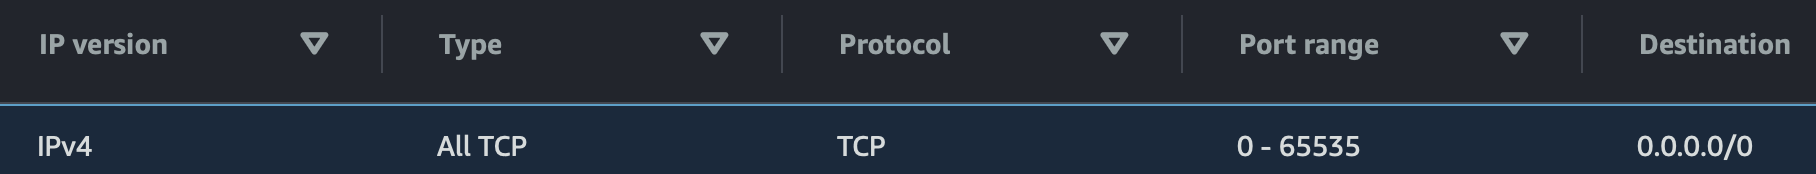
\includegraphics[width=\textwidth]{securityGroup2}
            \caption{security Group 2, TCP in uscita}
            \label{fig:sec2}
        \end{figure}
    \end{itemize}
\end{enumerate}


Una volta creata la macchina avremo la possibilità di scaricare la chiave privata con formato \lstinline{*.pem} che useremo per connetterci tramite SSH alla shell della macchina
\begin{lstlisting}[caption={Connessione SSH}]
    ssh -i key.pem admin@*.compute.amazonaws.com
\end{lstlisting}
La primissima operazione sarà l'aggiornamento dei repository e del sistema
\begin{lstlisting}[caption={Aggiornamento del sistema}]
    sudo apt update && sudo apt full-upgrade -y
\end{lstlisting}

Poi installiamo il web server nginx che abbiamo analizzato prima
\begin{lstlisting}[caption={Installazione Nginx}]
    sudo apt install nginx
\end{lstlisting}

Una volta completata l'installazione il web server viene automaticamente avviato e messo in ascolto sulla porta 80, in caso non fosse attivo \\
\begin{lstlisting}[caption={Avvio di Nginx}]
    sudo systemctl start nginx
\end{lstlisting}

Per installare tor è innanzitutto necessario installare \textbf{apt-transport-https} per utilizzare i repository tramite HTTPs
\begin{lstlisting}
    sudo apt install apt-transport-https
\end{lstlisting}
Dal comando \lstinline{lsb_release -c} possiamo vedere la distribuzione corrente e inserire il repository corretto nella configurazione, con Debian 11 siamo su di una distrubuzione bullseye, creiamo un file chiamato \lstinline{tor.list} \footnote{Il nome è configurabile} nella cartella \lstinline{/etc/apt/sources.list.d} dove andremmo ad aggiungere i repository TOR tramite le seguenti righe
\begin{lstlisting}[caption={Tor Repository}]
    deb [signed-by=/usr/share/keyrings/tor-archive-keyring.gpg] https://deb.torproject.org/torproject.org bullseye main
    deb-src [signed-by=/usr/share/keyrings/tor-archive-keyring.gpg] https://deb.torproject.org/torproject.org bullseye main
\end{lstlisting}

Assicuriamoci che GPG sia installato nel sistema prima di aggiungere le chiavi
\begin{lstlisting}[caption={Installazione GPG}]
    sudo apt install gpg
\end{lstlisting}

Aggiungiamo le chiavi GPG della repository appena creata
\begin{lstlisting}[caption={Aggiunta chiavi gpg dal repository Tor}]
    wget -qO- https://deb.torproject.org/torproject.org/A3C4F0F979CAA22CDBA8F512EE8CBC9E886DDD89.asc | gpg --dearmor | tee /usr/share/keyrings/tor-archive-keyring.gpg >/dev/null
\end{lstlisting}

Aggiorniamo gli index e installiamo finalmente tor
\begin{lstlisting}[caption={Installazione Tor}]
    sudo apt update && sudo apt install tor -y 
\end{lstlisting}

\cite{TorRepo}

Generiamo il file \lstinline{torrc} che ci servirà per impostare tutti i parametri di configurazione 
\begin{lstlisting}[caption={Generazione file torrc}]
    sudo tor -f /etc/tor/torrc
\end{lstlisting}

Apriamo il file \lstinline{/etc/tor/torrc} e togliamo il commento alle righe \lstinline{HiddenServicePort 80 127.0.0.1:80} e \lstinline{HiddenServiceDir /var/lib/tor/hidden_service}, il primo indica che il traffico arrivato dalla porta virtuale (80) viene reindirizzato alla porta 80 del localhost, ovvero la porta in cui è in ascolto il web server nginx, il secondo ci serve per indicare la directory in cui salvare l'hostname del sito e le chiavi crittografiche, o eventualmente la directory in cui sono già presenti. \\
Riavviamo tor per aggiornare la configurazione, assicurarci che il file torrc non contenga errori e che il sistema sia funzionante
\begin{lstlisting}
    sudo systemctl restart tor
\end{lstlisting}

\subsection{Gestire la comunicazione tramite i socket unix}
A questo punto tor ha creato gli introduction points e ha generato un circuito con ognuno di essi, ha inoltre generato le chiavi e il proprio hostname, queste informazioni sono state aggiunte nella cartella che abbiamo inserito nell'HiddenServicePort, in particolare il file chiamato hostname contiene l'indirizzo tor del nostro servizio \cite{SetupOnionService} \\
Questo sistema però non è completamente sicuro, infatti Tor è connesso con il web server tramite la porta 80, essendo entrambi i processi sulla stessa macchina il sistema ottimale è utilizzare un socket unix tra i due processi. 
Questo impedisce a un utente \textbf{non} Tor di accedere direttamente al web server senza dover configurare un firewall che comunque aggiunge complessità nella rete. \\
Apriamo il file \lstinline{/etc/nginx/sites-enabled/default} e nella sezione server aggiungiamo il socket in ascolto, cosi che la comunicazione possa passare anche per il socket unix
\begin{lstlisting}[caption={Aggiunta/creazione socket unix}]
    listen unix:/var/run/website.sock;
\end{lstlisting}

Possiamo inoltre rimuovere la connessione dalla porta 80 commentando le seguenti righe
\begin{lstlisting}[caption={Rimozione connessione dalla porta 80}]
    #listen 80 default_server;
    #listen [::]:80 default_server;
\end{lstlisting}

Dopo aver riavviato nginx ed esserci assicurati che non vi siano errori apriamo il file torrc e inseriamo lo stesso socket
\begin{lstlisting}[caption={Aggiunta socket unix a torrc}]
    HiddenServicePort 80 unix:/var/run/website.sock
\end{lstlisting}

Infine riavviamo tor
\begin{lstlisting}
    sudo systemctl restart tor
\end{lstlisting}
Se tutto è andato a buon fine il web server non dovrebbe essere in grado di rispondere alle richieste HTTP dalla porta 80, ma solo a quelle provenienti dalla rete Tor tramite l'hostname .onion che abbiamo ricevuto precedentemente. \\
\importImage{
    \label{fig:nginxConnection} 
    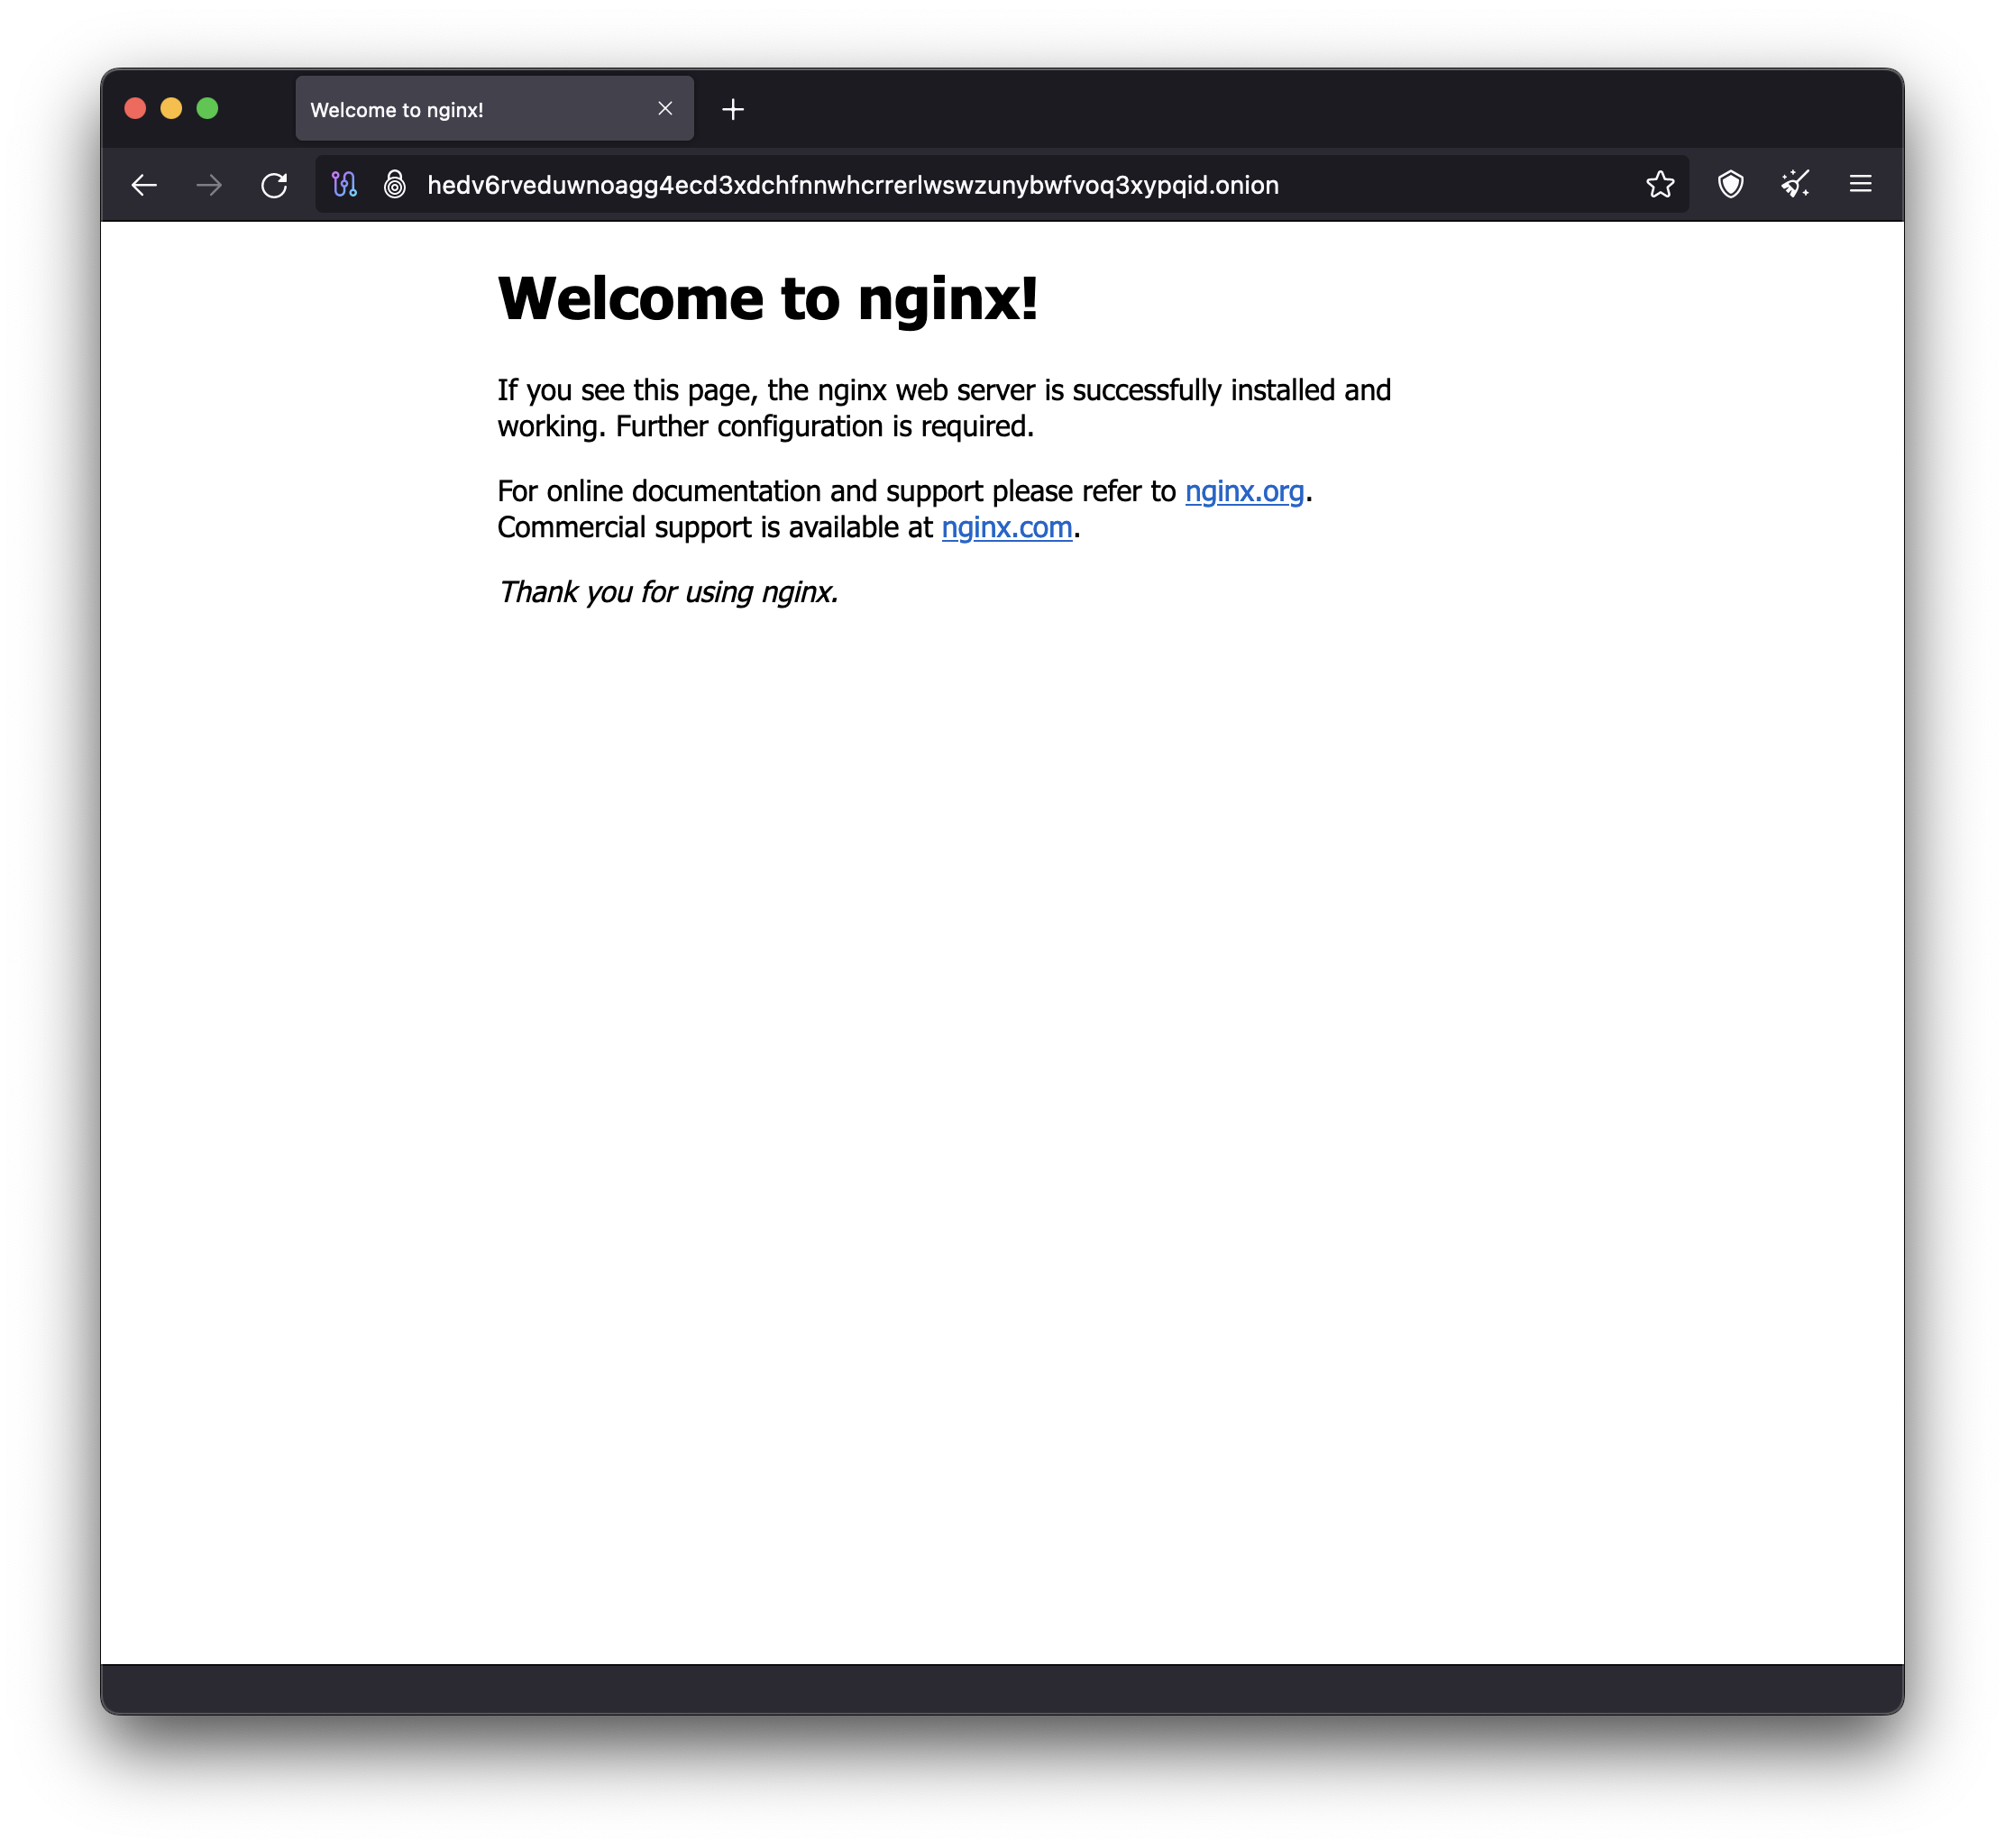
\includegraphics[width=\textwidth]{connectionSucceeded}
    \caption{Connessione al web server nginx}
}

\newpage
\subsection{Creazione di un url personalizzato}
Ora che il servizio è attivo e disponibile possiamo iniziare a configurarlo a nostro piacimento, la prima cosa che potremmo voler fare è cambiare l'hostname impostandone uno personalizzato, almeno in parte, un esempio è il sito email di proton \textbf{protonmail}rmez3lotccipshtkleegetolb73fuirgj7r4o4vfu7ozyd.onion \\
Si sfrutta la tecnica del brute force per generare coppie di chiavi casuali da cui ottenere indirizzi .onion fino a che non ne troviamo uno che inizia con la stringa che abbiamo scelto, potrebbe impiegare diverso tempo ed è consigliabile usare un computer più potente della nostra macchina virtuale. 
Vi sono diversi strumenti per fare quest'operazione sia v2 che v3, per questa implementazione useremo il tool mkp224o \cite{V3AddressGeneratorRepo} che appunto ci permette di fare quest'operazione con gli indirizzi v3, possiamo installarlo su Linux o usarlo su Windows da riga di comando semplicemente indicando il nome con cui dovrà iniziare

\begin{lstlisting}
    ./mkp224o tesilm
\end{lstlisting}
\footnote{Il file viene avviato direttamente dalla cartella del sorgente, per cui apponiamo \lstinline{./}}

Da notare che più caratteri si scelgono nel matching più il software impiegherà nella generazione di un dominio. 
Otteniamo il nuovo indirizzo del servizio\footnote{tesilm3jb64lw3upj4uu5fsxi2nrtbhbhkbu2dsbn46qka7j4kf7peqd.onion} con le relative chiavi \\
Possiamo copiarle sul server con SCP usando l'opzione -i per definire il file d'identità, come facciamo con SSH

\begin{lstlisting}
    cd tesilm3jb64lw3upj4uu5fsxi2nrtbhbhkbu2dsbn46qka7j4kf7peqd.onion
    scp -i key.pem * admin@*.compute.amazonaws.com:~/var/lib/tor/hidden_service
\end{lstlisting}

Avviamo la connessione al server e riavviamo tor per impostare le modifiche

\importImage{
    \label{fig:mkpCommandOut} 
    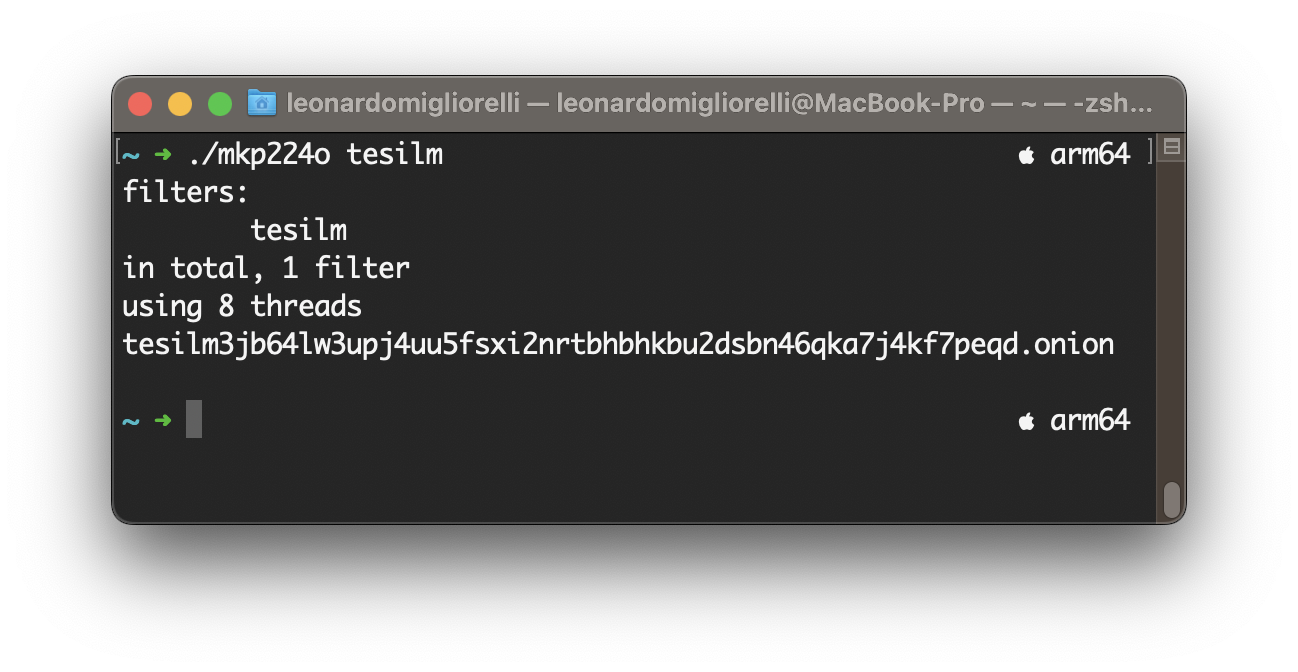
\includegraphics[width=\textwidth]{mkpCommandOut}
    \caption{Comando mkp224o e output}
}

\importImage{
    \label{fig:customAddressConnection} 
    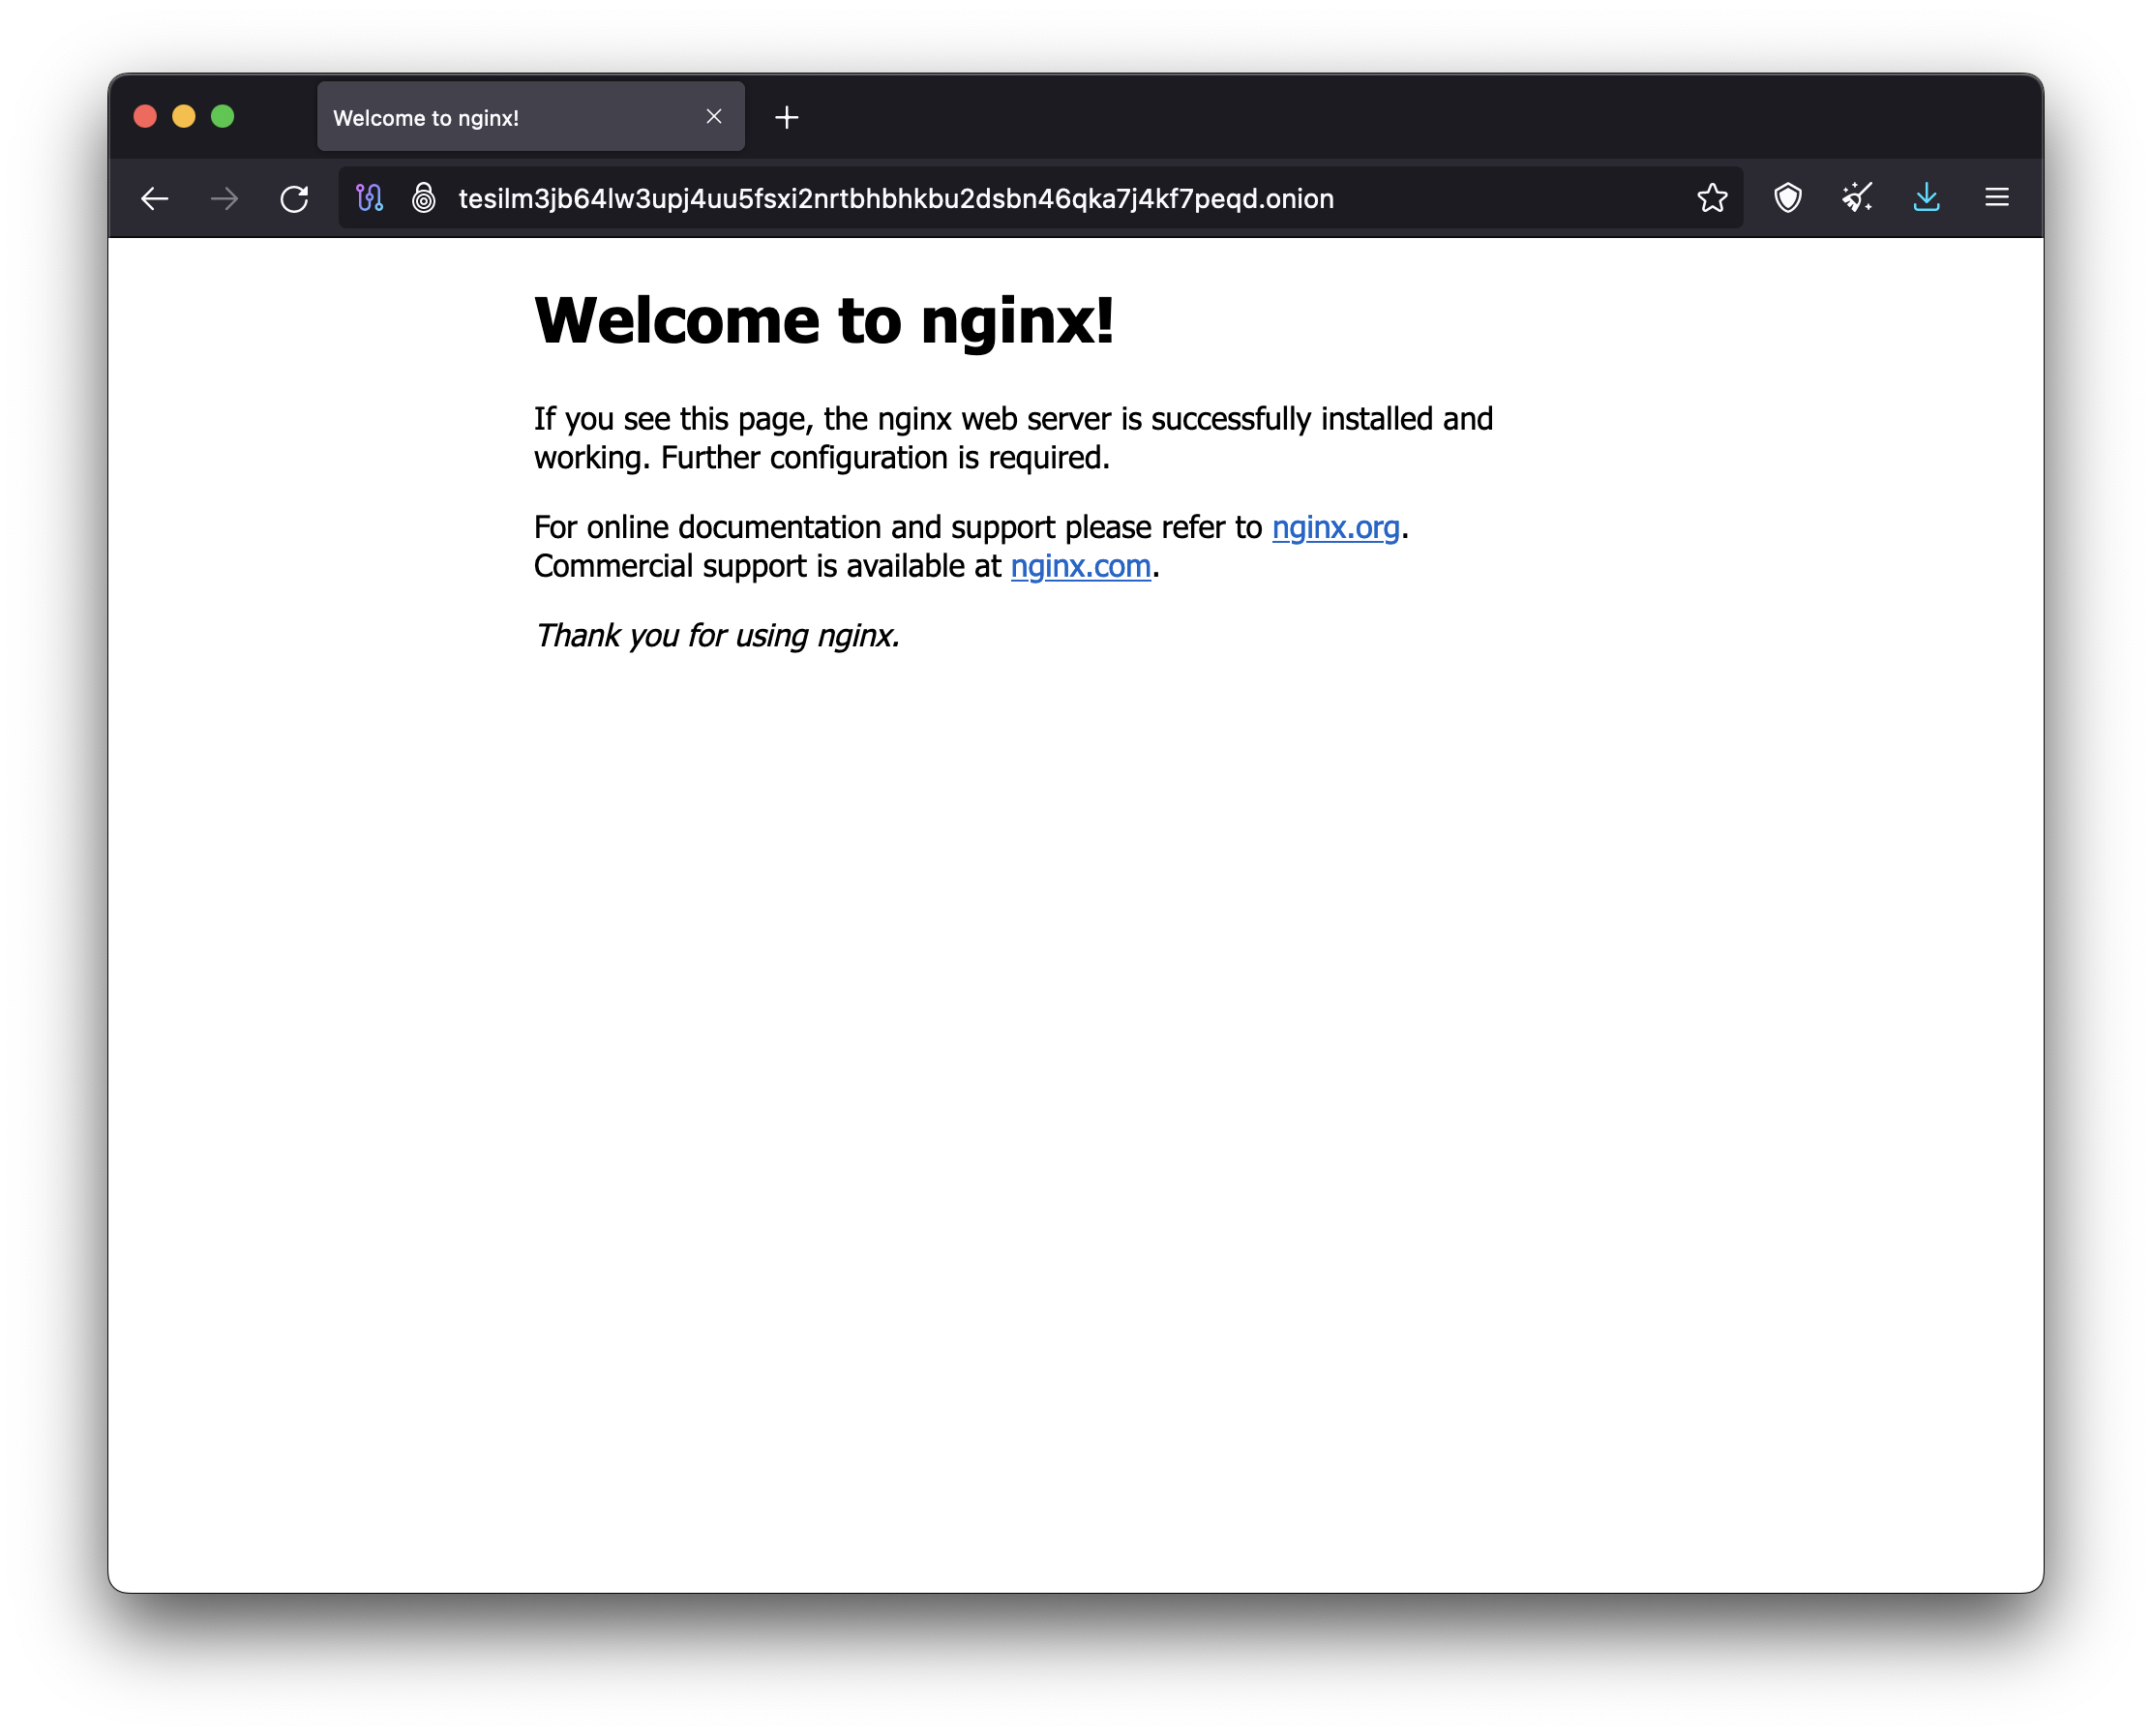
\includegraphics[width=\textwidth]{connectionCustomAddress}
    \caption{Connessione con il nuovo URL}
}

\newpage

\subsection{Far conoscere il sito}
Un'altra caratteristica importante per ogni sito è la capacità di essere trovato dall'utente finale, solitamente tramite un motore di ricerca, ci sono diversi motori che eseguono l'indexing di indirizzi onion. Tra questi c'è notevil\footnote{http://notevilmtxf25uw7tskqxj6njlpebyrmlrerfv5hc4tuq7c7hilbyiqd.onion} funziona come un classico motore di ricerca, a differenza di altri motori come Torch che invece esegue la ricerca più in base al contenuto che all'url\footnote{Un test di ricerca di 'proton mail' in entrambi mostra solo notEvil restituirci il sito corretto} \\
In NotEvil è possibile contattare gli amministratori del motore per richiedere l'aggiunta di un sito. 
Dalla pagina ufficiale è infatti presente il pulsante di contatto, dopo un breve controllo ci permette di inviare una richiesta anonima cosi che il sito possa essere analizzato e aggiunto. \\
Un altro sistema per far conoscere il sito agli utenti finali è l'utilizzo di siti specializzati come OnionDir\footnote{https://oniondiricuc4x2y5qbucg4jyp2ael5rxy7aahy5f4fbars2jkkf7vad.onion.nz} che permette di aggiungere il proprio sito in maniera completamente anonima. \\
In questo caso basta cliccare sul tasto \lstinline{Add Link} nella toolbar in alto. \\
\importImage{
    \label{fig:OnionDir}
    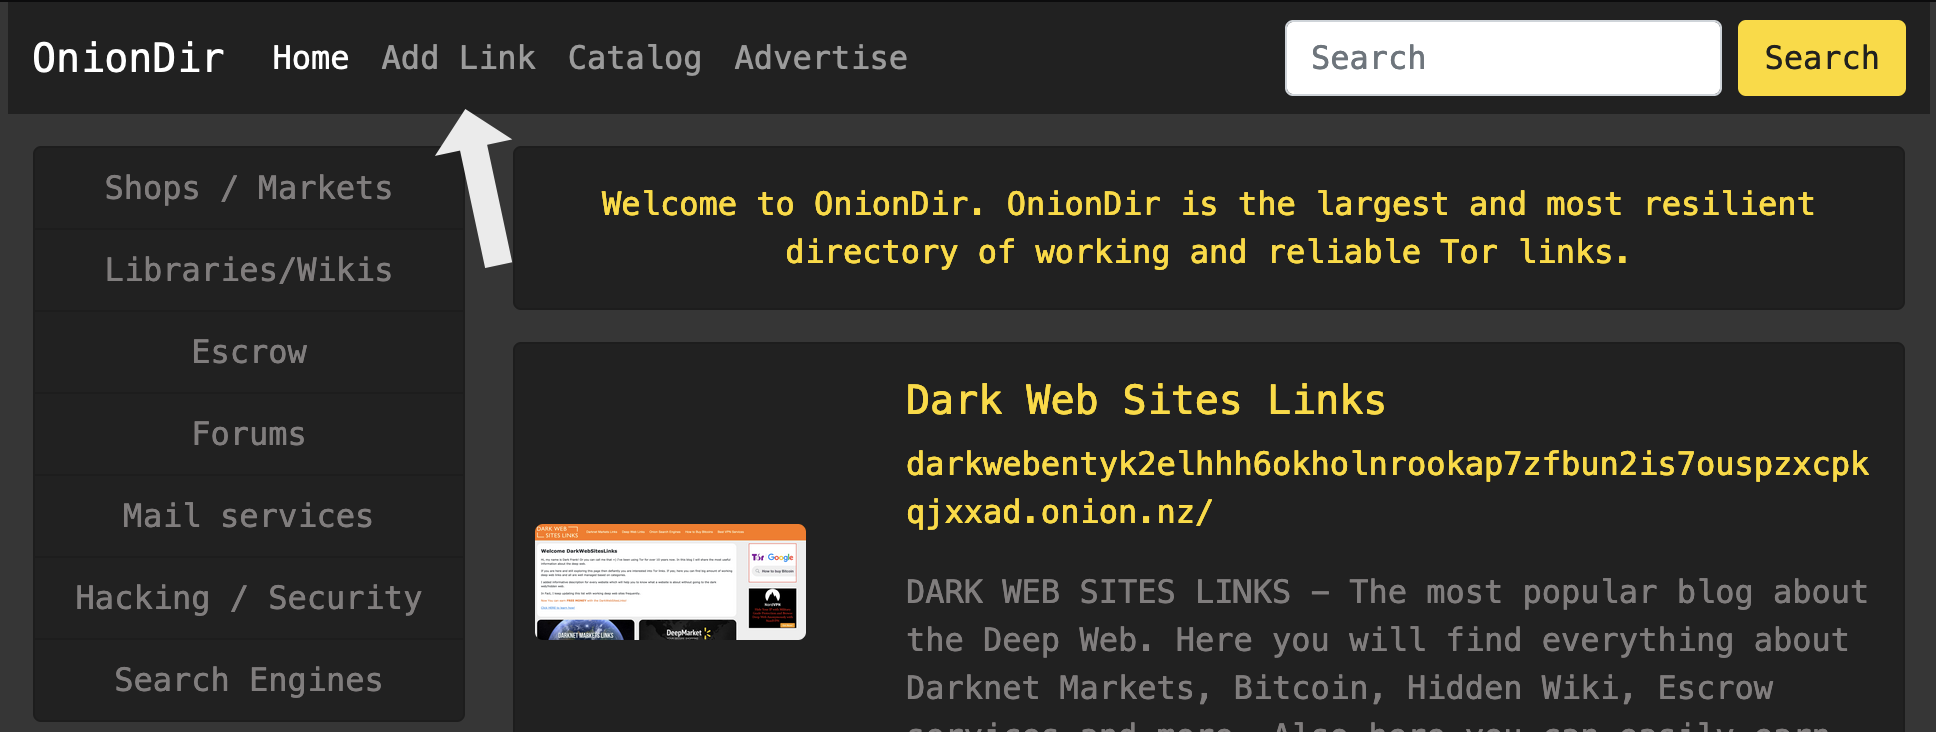
\includegraphics[width=\textwidth]{OnionDirMain}
    \caption{OnionDir, Pagina iniziale}
}
A questo punto possiamo inserire l'URL e una piccola descrizione, come NotEvil il sito sarà scansionato per evitare truffe o contenuti proibiti, come indicato nelle poche righe di descrizione dei termini del servizio. \\
\importImage{
    \label{fig:OnionDirForm}
    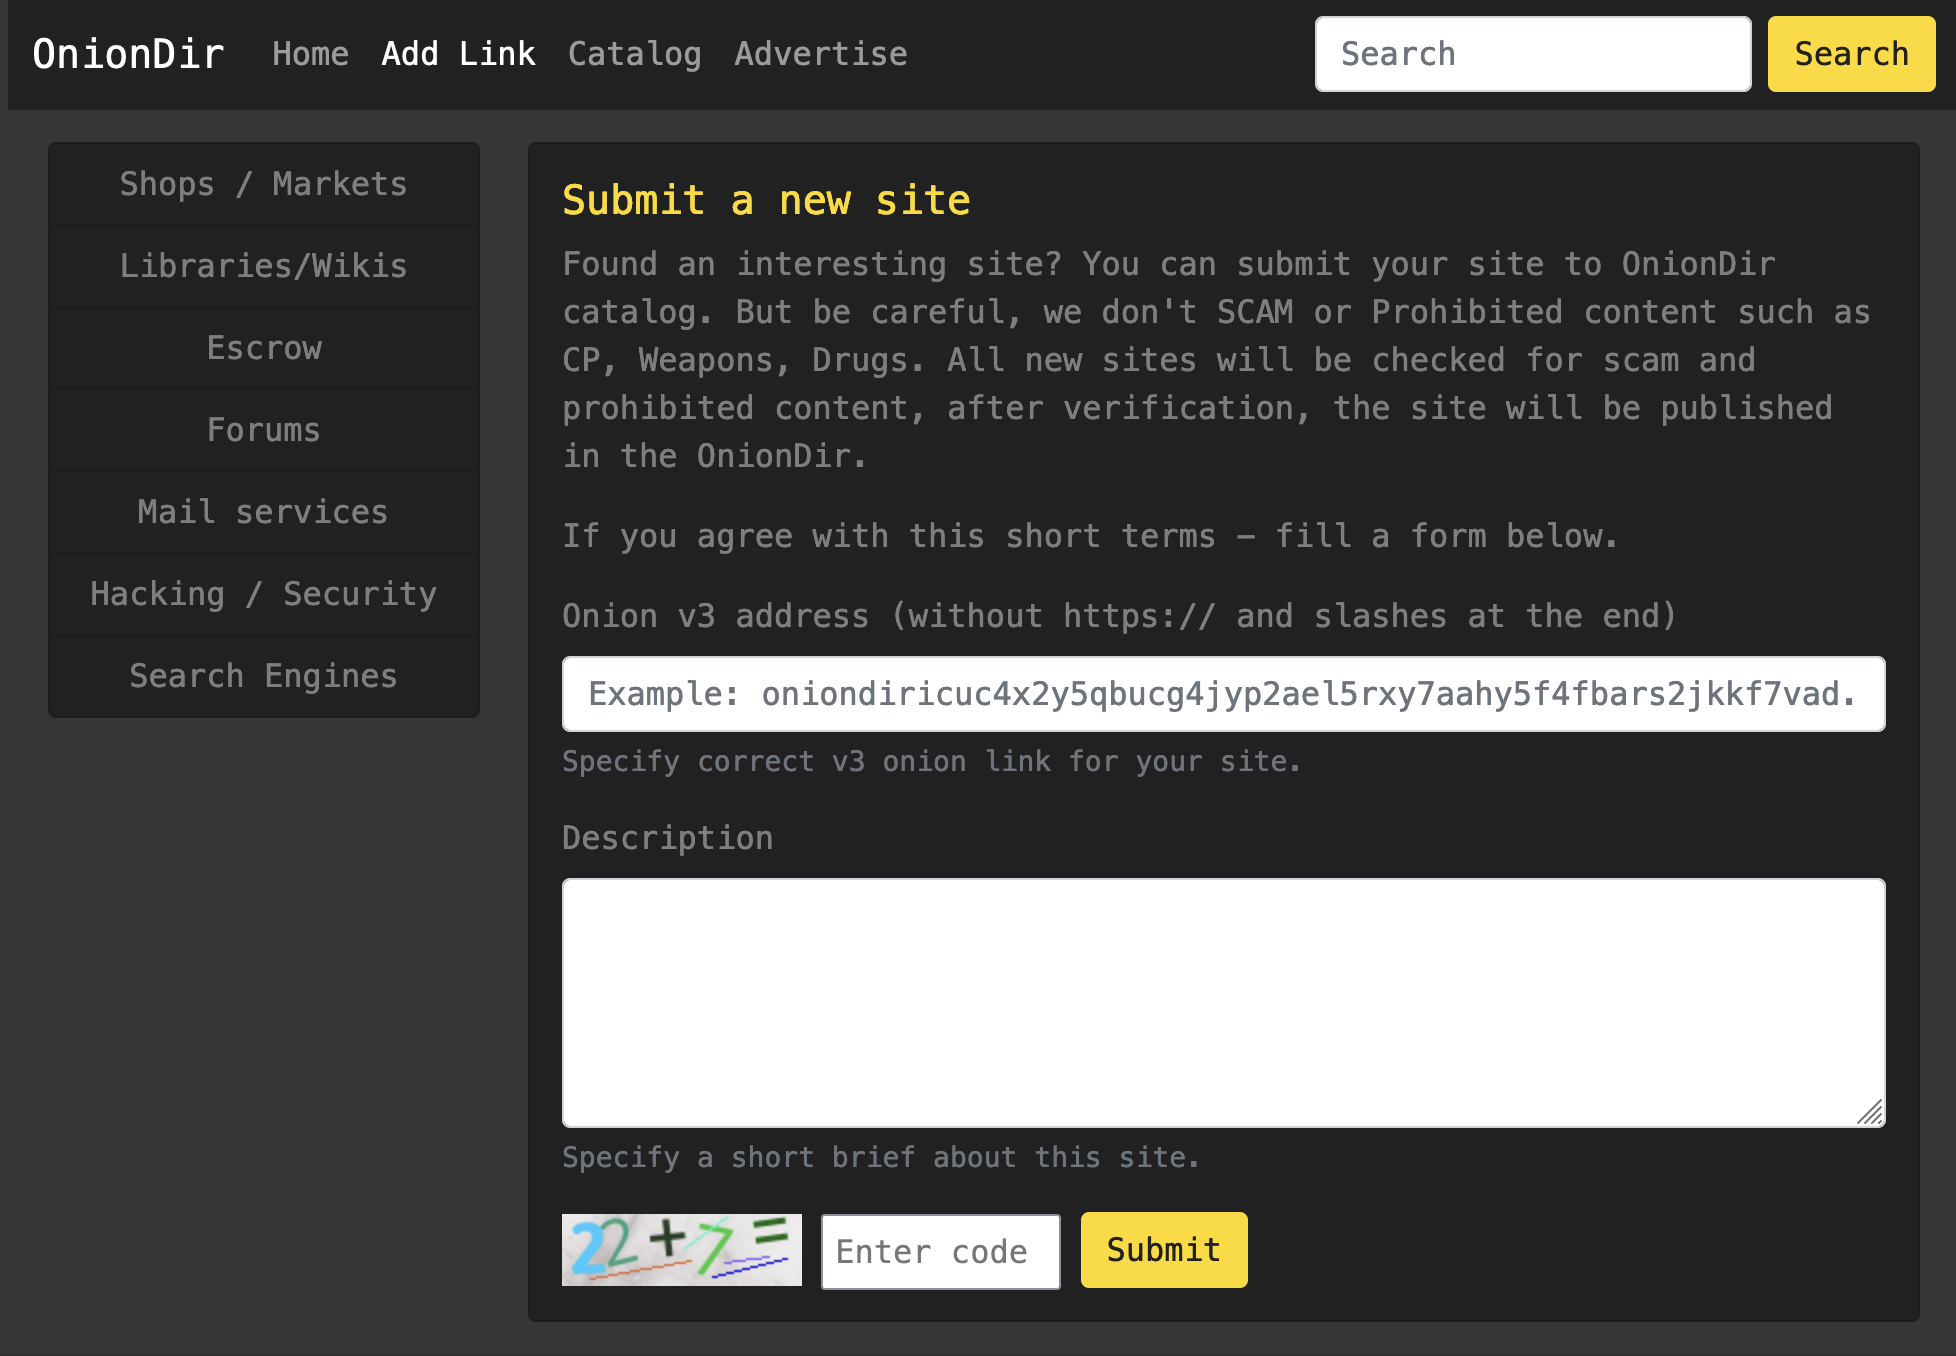
\includegraphics[width=\textwidth]{OnionDirForm}
    \caption{OnionDir, form aggiunta sito}
}
\newpage
Un altro sistema per far conoscere il sito è tramite il cosiddetto \emph{Onion-Location Header} che permette di indicare al browser che il sito è disponibile anche su Tor, in questo modo quando la pagina viene visitata il browser può mostrare un pulsante per aprire il sito direttamente su Tor. \\
Il miglior esempio è il sito ufficiale di \href{www.torproject.org}{Tor Project} che mostra un pulsante per aprire il sito onion quando viene visitato tramite la rete Tor\footnote{Da tenere in considerazione che questo metodo richiede un sito normale per funzionare}. \\
\importImage{
    \label{fig:TorProjectOnionAvailable}
    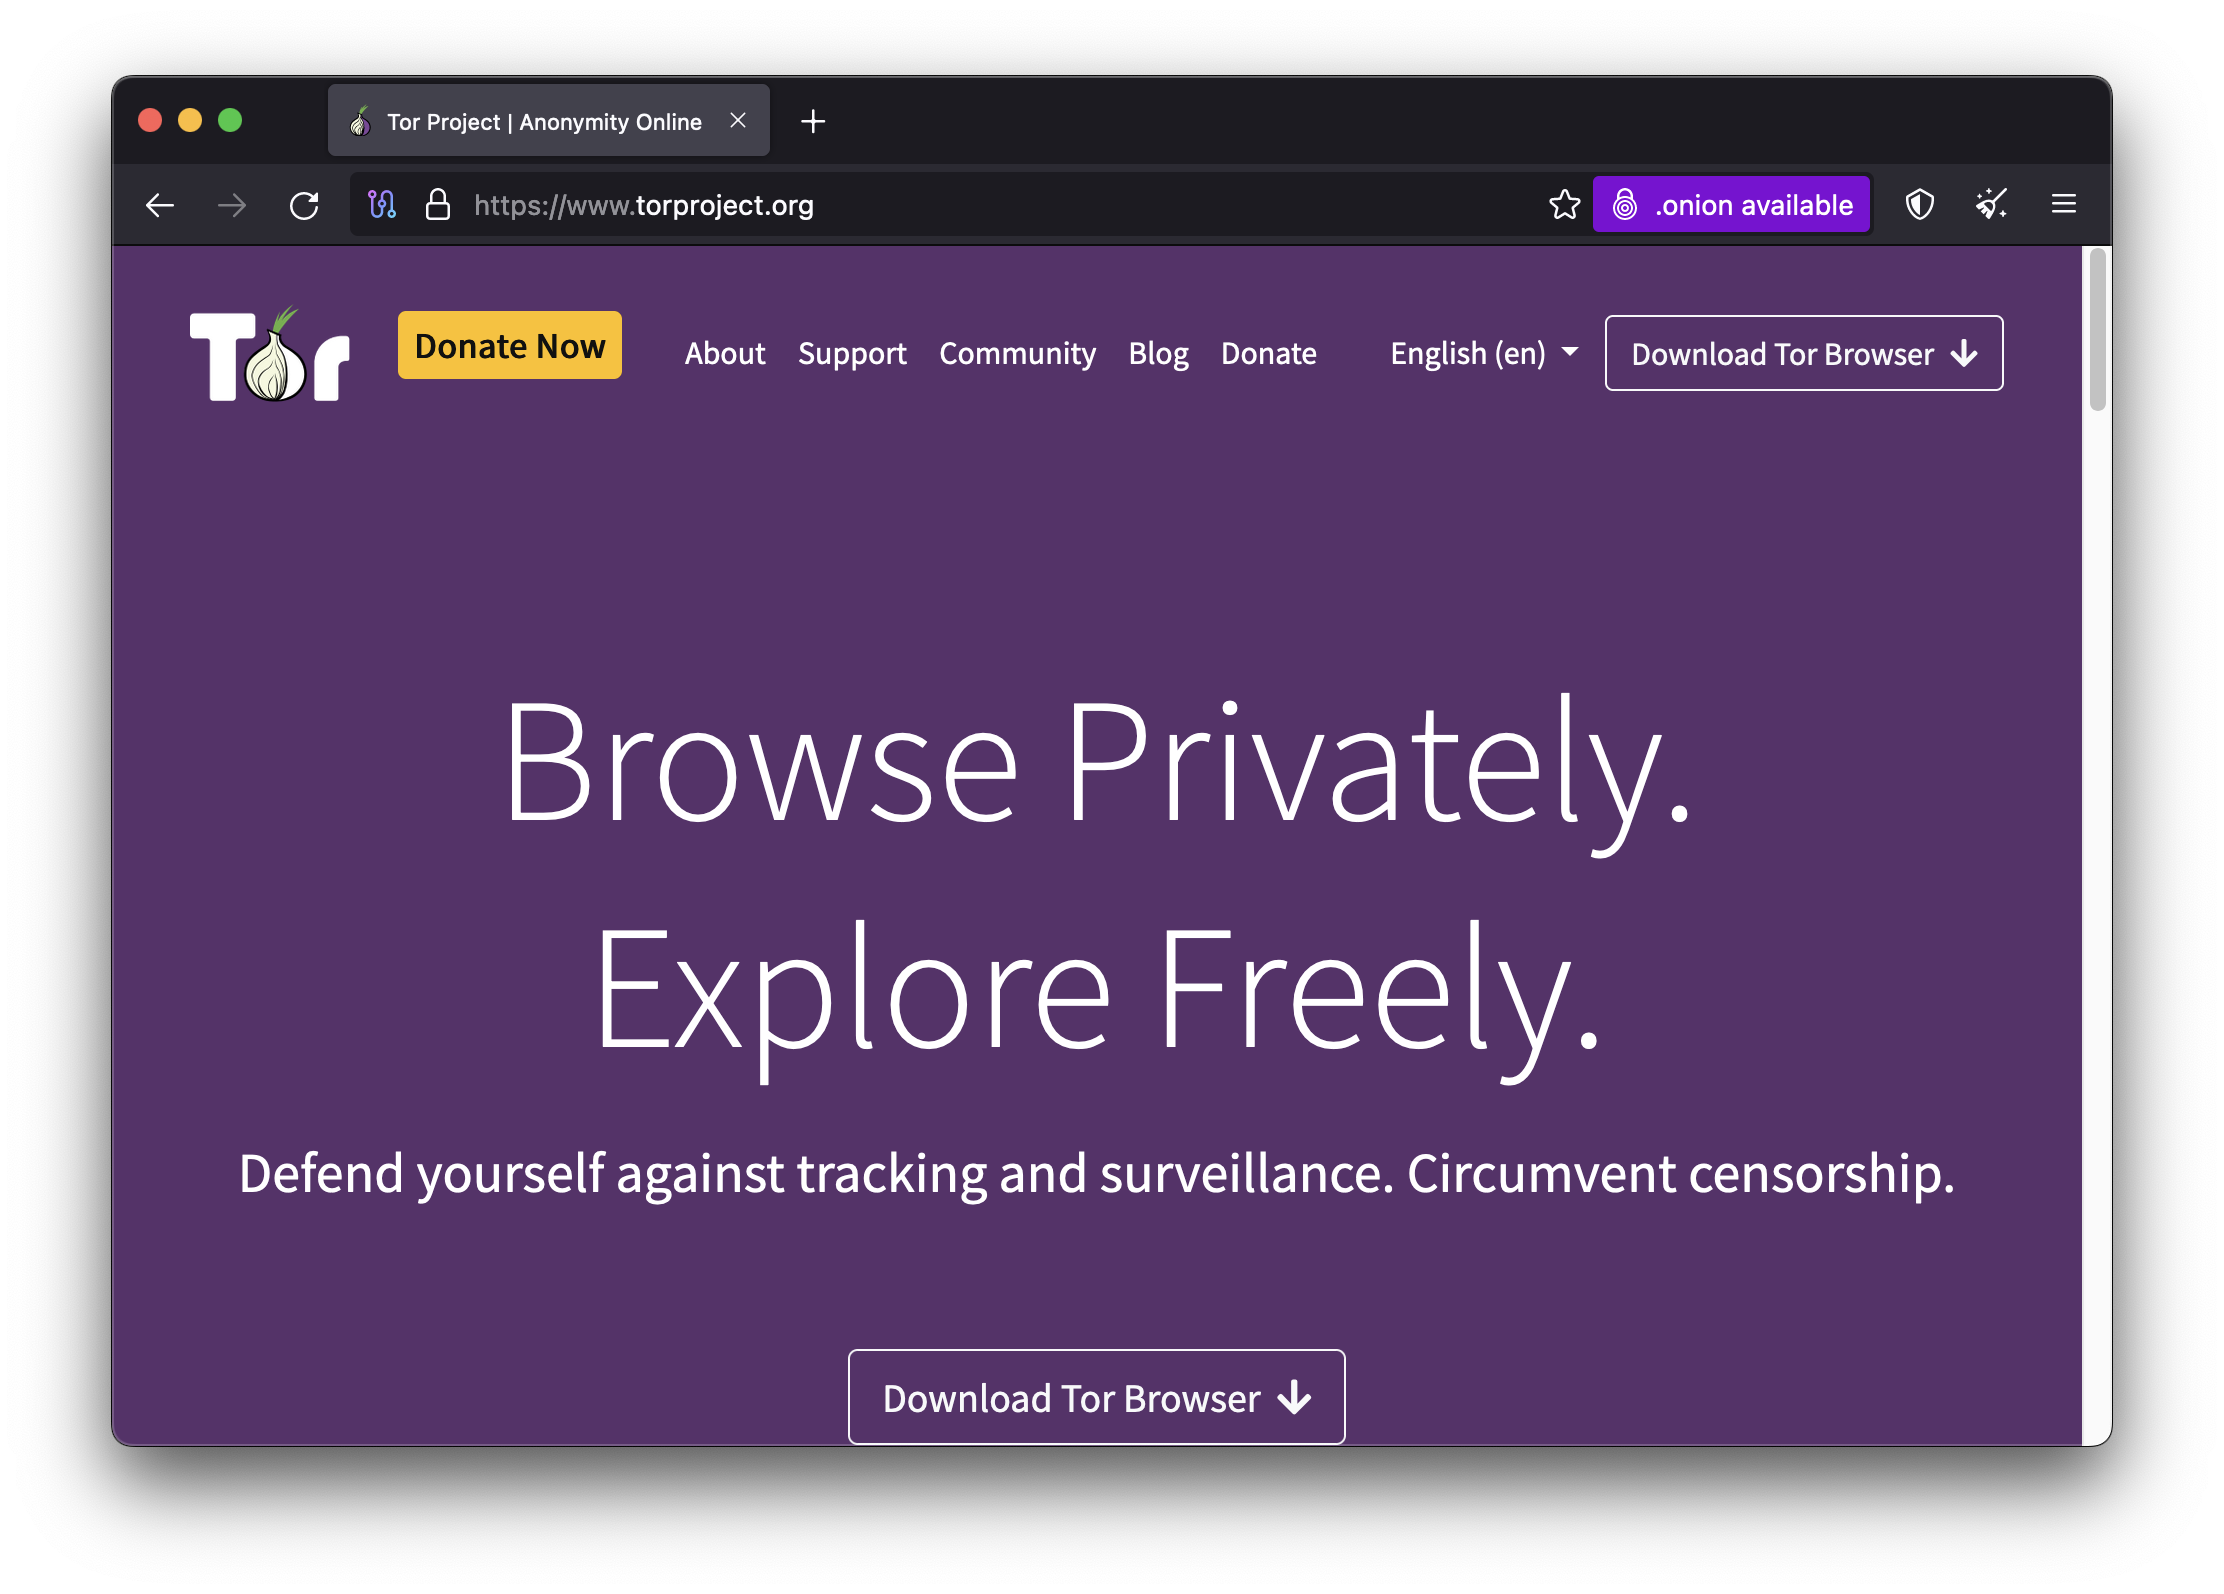
\includegraphics[width=\textwidth]{TorProjectOnionAvailable}
    \caption{Tor Browser mostra il pulsante \emph{.onion available} quando si visita il sito tramite Tor}
}

\newpage
Per aggiungere questo header è sufficiente aggiungere la seguente riga al file di configurazione del server
\begin{lstlisting}
    add_header Onion-Location http://tesilm3jb64lw3upj4uu5fsxi2nrtbhbhkbu2dsbn46qka7j4kf7peqd.onion$request_uri;
\end{lstlisting}
\footnote{Il tag \lstinline{$request_uri} indica la sotto-pagina corrente, e quindi la pagina in cui andremo a fare il redirect, questa operazione non può essere fatta inserendo direttamente il tag all'interno del file HTML, in quanto non è possibile leggere l'url corrente della pagina}
Oppure possiamo aggiungere direttamente il tag \lstinline{<meta>} nella sezione header della pagina HTML, nel caso di configurazioni particolari
\begin{lstlisting}[language=HTML]
    <meta http-equiv="onion-location" content="http://tesilm3jb64lw3upj4uu5fsxi2nrtbhbhkbu2dsbn46qka7j4kf7peqd.onion" />
\end{lstlisting}
Questo metodo però ha un problema, non potendo leggere l'url della pagina corrente il tag \lstinline{<meta>} esegue sempre il redirect alla home page, indipendentemente dalla sotto-pagina corrente. 
L'unico modo per risolvere questo problema è inserire manualmente il tag in ogni sottopagina ed inserire il path nell'indirizzo onion del tag. \\
L'implementazione di questa seconda tecnica è stata mostrata nel mio sito \href{https://tesi.miglio.dev}{tesi.miglio.dev} che mostra il pulsante per aprire il sito onion quando viene visitato tramite Tor. \\
\importImage{
    \label{fig:ClearWebPage}
    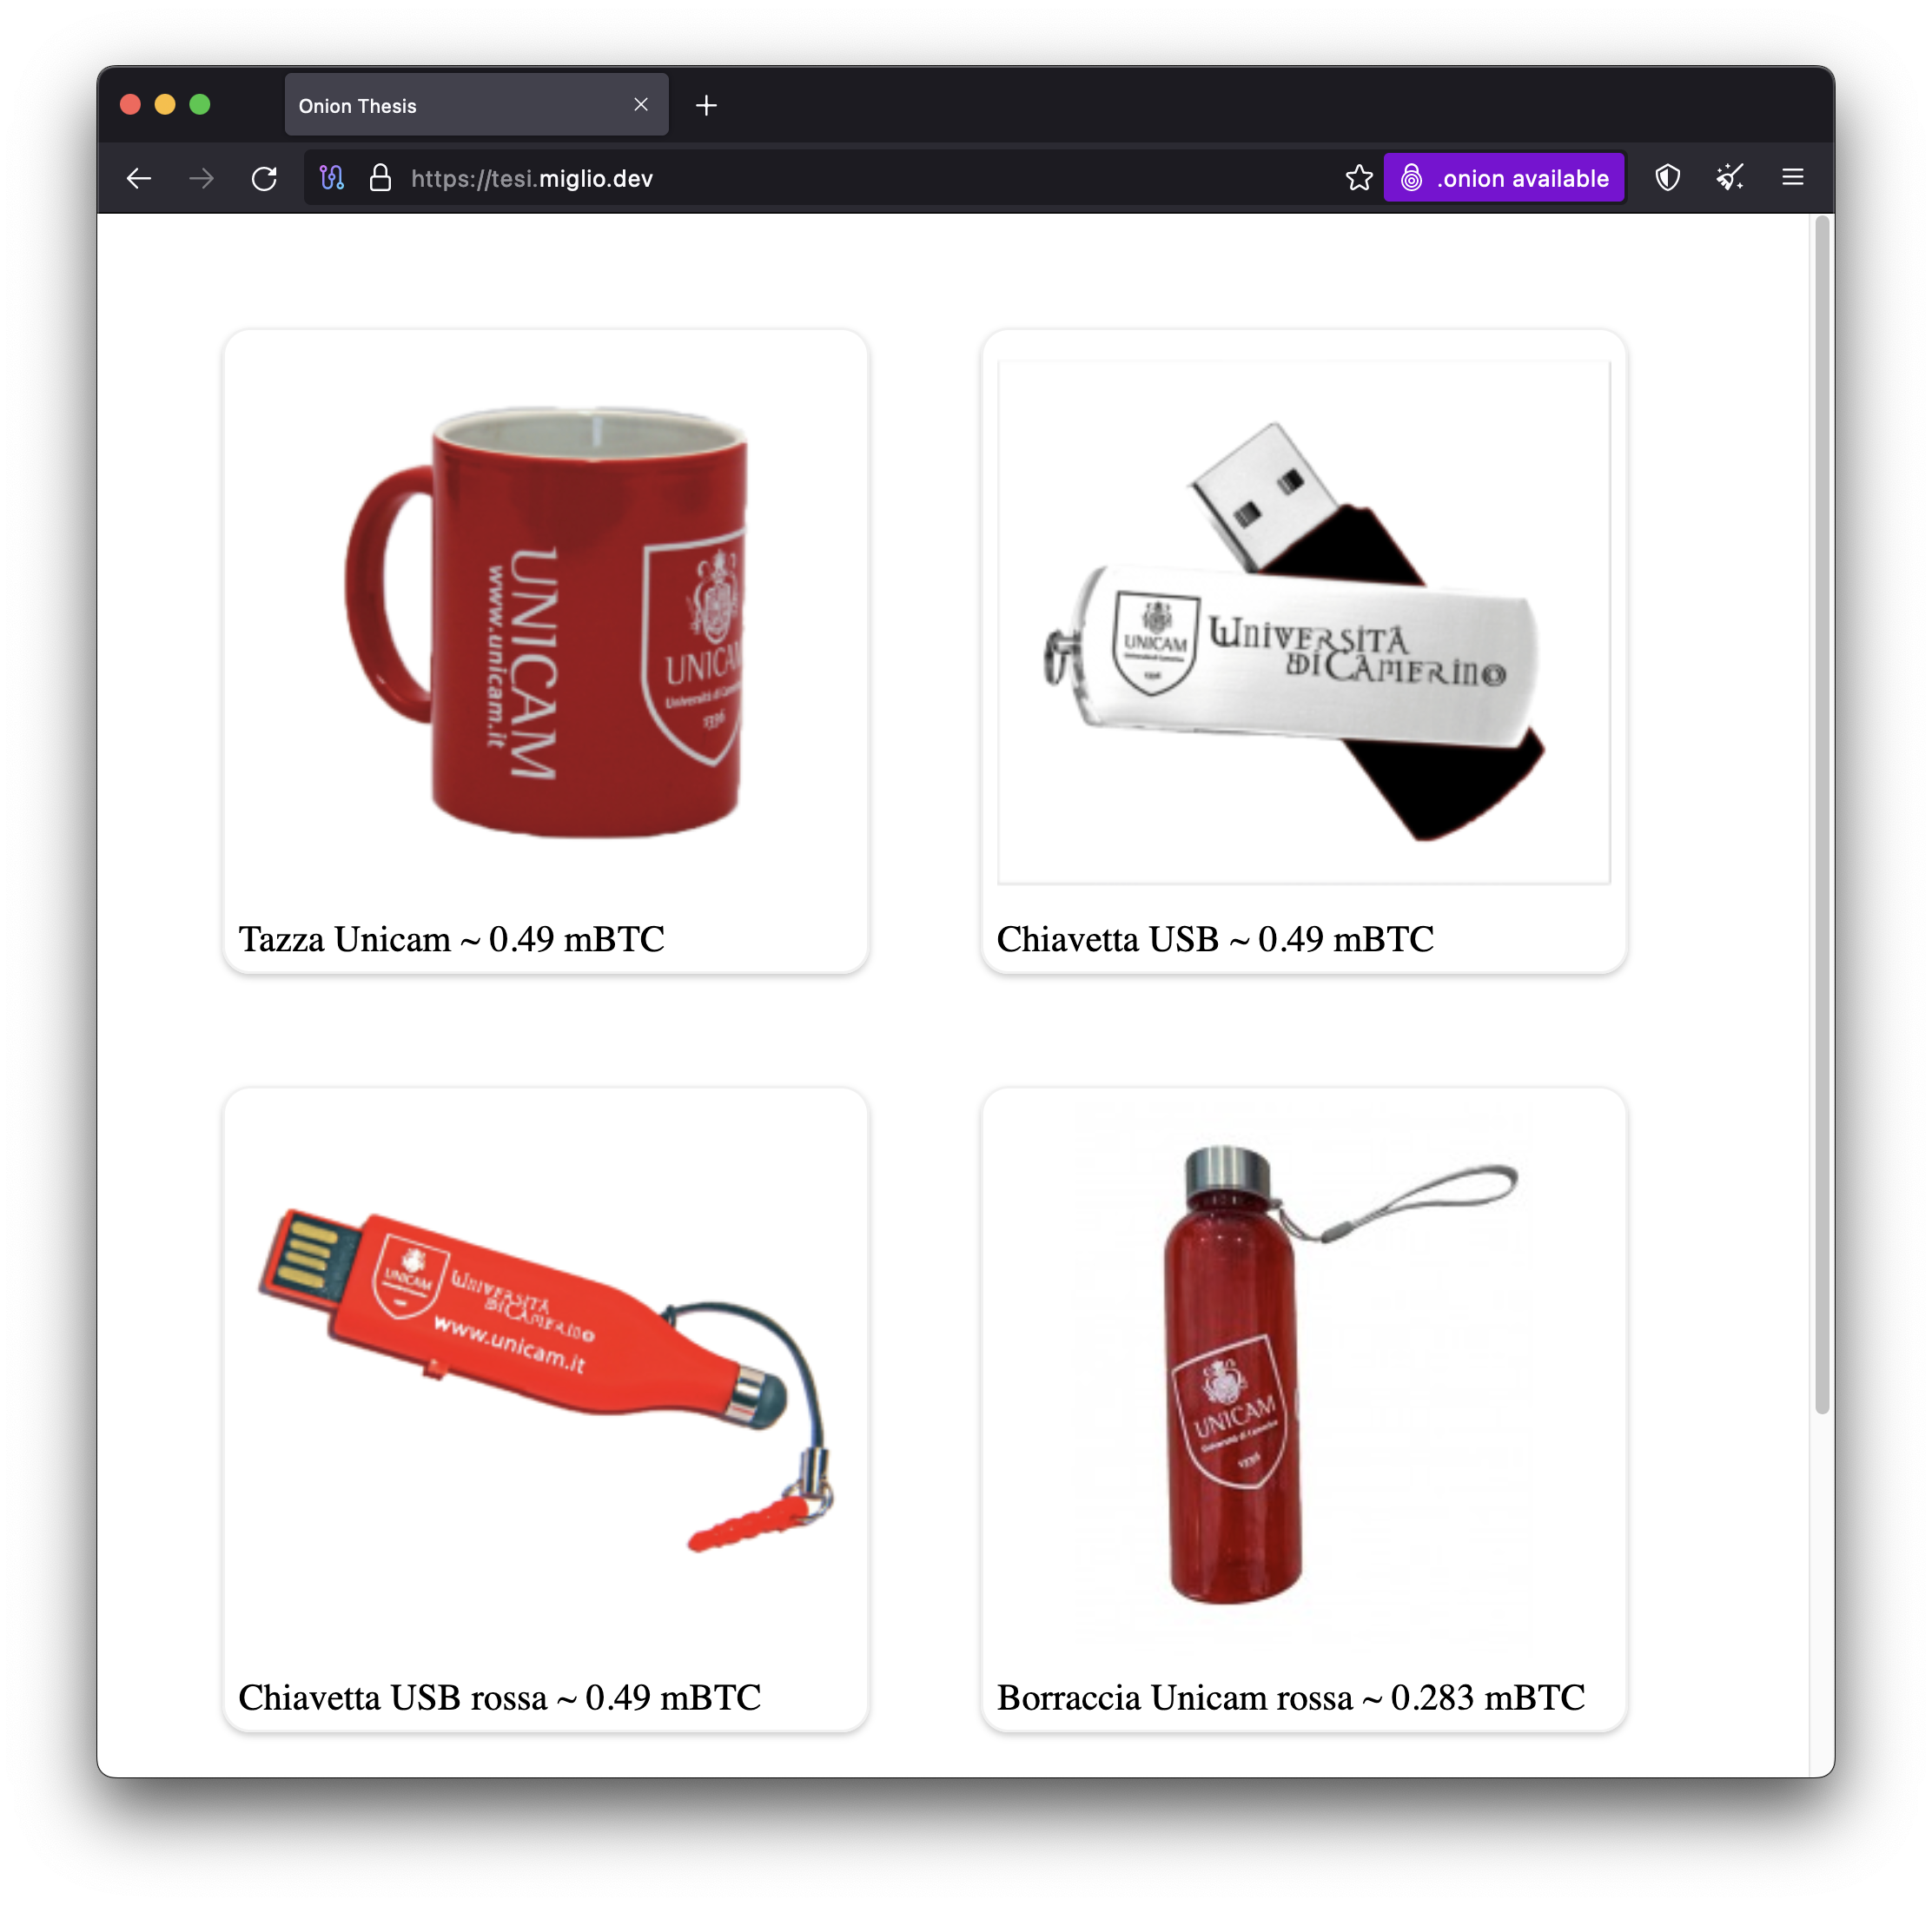
\includegraphics[width=\textwidth]{ClearWebPage}
    \caption{Tor Browser mostra il pulsante \emph{.onion available} quando si visita il nostro sito tramite Tor}
}
\cite{OnionLocationHeader}